
\documentclass[border={0pt 0pt 0pt 0pt}]{standalone}
\usepackage{tikz-cd,tikz-3dplot} 
\usetikzlibrary{calc,intersections,through,backgrounds,decorations.pathmorphing, decorations.shapes,decorations.markings,patterns}
%include other needed packages here   
\begin{document}
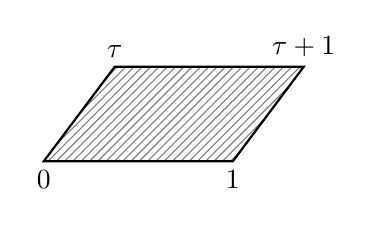
\begin{tikzpicture}[scale=3]
\fill [pattern=north east lines, pattern color=gray] (0,0) -- (0.8,0) -- (1.1,0.4) -- (0.3,0.4) -- (0,0);
\foreach \x/\xtext in {0/0,0.8/1}
\draw  (\x,0) node[anchor=north,fill=white] {$\xtext$};
\foreach \x/\xtext in {0.3/\tau,1.1/\tau+1}
\draw  (\x,0.4) node[anchor=south,fill=white] {$\xtext$};
\draw[thick] (0,0) -- (0.8,0) -- (1.1,0.4) -- (0.3,0.4) -- cycle;
\end{tikzpicture}
\end{document}